\documentclass[11pt,a4paper]{article}
\usepackage[T1]{fontenc}
\usepackage[utf8]{inputenc}
\usepackage[magyar]{babel}
\usepackage{lmodern}
\usepackage{amsmath,amssymb}
\usepackage{enumitem}
\usepackage{tikz}
\usetikzlibrary{arrows.meta}
\usepackage[a4paper,margin=2cm]{geometry}

\pagestyle{empty}
\setlength{\parindent}{0pt}
\setlist[enumerate,1]{label=\textbf{\arabic*.}, leftmargin=*, itemsep=10pt, topsep=3pt}
\setlist[enumerate,2]{label=\alph*), leftmargin=2em, itemsep=4pt, topsep=3pt, parsep=0pt}

\begin{document}

\begin{center}
  {\Large\bfseries Termodinamika -- összefoglaló feladatok -- megoldókulcs}\\[4pt]
  \fbox{\parbox{0.8\textwidth}{\centering
    $\Delta E = Q + W$, ahol $W$ a gázon végzett munka.}}
\end{center}

\begin{enumerate}
\item \textbf{Igaz vagy hamis?}
  \begin{enumerate}
    \item \textbf{Hamis.} Izoterm tágulásnál a gáz hőt vesz fel, de a hőmérséklete
      állandó, mert a felvett hővel egyenlő munkát végez. (Olvadó jég: szintén.)
    \item \textbf{Hamis.} Adiabatikusnál $Q = 0$, de $W \neq 0$, így $\Delta E = W \neq 0$:
      összenyomáskor melegszik, táguláskor hűl a gáz.
    \item \textbf{Hamis.} A belső energia állapotjelző, megváltozása csak a kezdő- és
      végállapottól függ. Az úttól $Q$ és $W$ függ.
    \item \textbf{Hamis.} $\Delta E_\text{össz} = 0$, de $Q_\text{össz} = -W_\text{össz}$,
      ami a hurok területe, nem nulla. (Hőerőgépnél éppen ez a hasznos munka.)
    \item \textbf{Igaz.} $\Delta E$ ugyanannyi, de állandó nyomáson a gáz kitágul és
      munkát végez, ehhez még $p\Delta V$ hő kell; $c_p - c_V = R$.
    \item \textbf{Hamis.} A belső energia nő: a közölt hő a kristályrács kötéseinek
      felbontására fordítódik. ($E$ csak ideális gáznál függ kizárólag $T$-től.)
    \item \textbf{Hamis.} Súrlódás nélkül is kell hideg tartály, ahová hőt ad le
      (II.~főtétel); a hatásfok legfeljebb $1 - T_\text{h}/T_\text{m} < 1$.
    \item \textbf{Hamis.} A többlethőt a hideg környezetből szivattyúzza át:
      $Q_\text{le} = W + Q_\text{fel}$, az energia megmarad.
  \end{enumerate}

\item $p_0V_0 = 10^5~\text{Pa}\cdot 3\cdot 10^{-3}~\text{m}^3 = 300~\text{J}$; egyatomos
  gázra $\Delta E = \tfrac32\,\Delta(pV)$.
  \begin{enumerate}
    \item $n = \dfrac{p_0V_0}{RT_A} = \dfrac{300}{8{,}31\cdot 300} \approx 0{,}12~\text{mol}$.\quad
      $T = \dfrac{pV}{nR}$, így $T_B = 2T_A = 600~\text{K}$, $T_C = 4T_A = 1200~\text{K}$.
    \item $A\to B$: izochor melegítés; $B\to C$: izobár tágulás; $C\to A$: egyik
      speciális folyamat sem. Az egyenes az origón megy át, tehát $p/V$ állandó; a gázt
      összenyomjuk, közben hűl.
      \begin{center}
      \renewcommand{\arraystretch}{1.45}
      \begin{tabular}{|l|c|c|c|}
      \hline
      Szakasz & $W$ & $\Delta E$ & $Q = \Delta E - W$ \\ \hline
      $A\to B$ & $0$ & $+\tfrac32\,p_0V_0 = +450~\text{J}$ & $+\tfrac32\,p_0V_0 = +450~\text{J}$ \\
      $B\to C$ & $-2p_0\cdot V_0 = -600~\text{J}$ & $+3\,p_0V_0 = +900~\text{J}$ & $+5\,p_0V_0 = +1500~\text{J}$ \\
      $C\to A$ & $+\tfrac{2p_0+p_0}{2}\cdot V_0 = +450~\text{J}$ & $-\tfrac92\,p_0V_0 = -1350~\text{J}$ & $-6\,p_0V_0 = -1800~\text{J}$ \\ \hline
      \textbf{Összesen} & $-\tfrac12\,p_0V_0 = -150~\text{J}$ & $0$ & $+\tfrac12\,p_0V_0 = +150~\text{J}$ \\ \hline
      \end{tabular}
      \end{center}
      ($C\to A$: a munka a trapéz alakú terület, pozitív, mert összenyomás.
      $B\to C$ ellenőrzés: $Q = \tfrac52 nR\,\Delta T = \tfrac52\cdot 2p_0V_0 = 5p_0V_0$.)
    \item $\tfrac32 + 3 - \tfrac92 = 0$. \checkmark
    \item A gáz az $A\to B$ és a $B\to C$ szakaszon vesz fel hőt. A $C\to A$ szakaszon
      végig hőt ad le, mert egyszerre nyomjuk össze ($W>0$) és hűl ($\Delta E<0$).
      $Q_\text{fel} = 450 + 1500 = 1950~\text{J}$.\\
      Hasznos munka: \textbf{1)} a munkák összegéből $W_\text{h} = 150~\text{J}$;
      \textbf{2)} a háromszög területéből $\tfrac12\cdot V_0\cdot p_0 = 150~\text{J}$.
      (Harmadik ellenőrzés: $Q_\text{fel} - |Q_\text{le}| = 1950 - 1800 = 150~\text{J}$.)\\
      $\eta = \dfrac{150}{1950} = \dfrac{1}{13} \approx 7{,}7\%$.
    \item $T_\text{max} = T_C = 1200~\text{K}$, $T_\text{min} = T_A = 300~\text{K}$:
      $\eta_\text{max} = 1 - \tfrac{300}{1200} = 75\%$. A mi gépünk ennek csak kb.\
      tizedét éri el. Ez nem sérti a II.~főtételt, de mutatja, hogy a körfolyamat messze
      van az ideálistól: a hőcsere nem csak a két szélső hőmérsékleten történik.
    \item A hőt mindkét körfolyamat ugyanazon a két szakaszon ($A\to B$, $B\to C$) veszi
      fel, a visszaút ($C\to D\to A$, illetve $C\to A$) pedig csak hőleadással jár. Ezért
      $Q_\text{fel} = \tfrac{13}{2}p_0V_0$ mindkét esetben. A bezárt terület viszont a
      téglalapnál $p_0V_0$, a háromszögnél csak $\tfrac12 p_0V_0$: az átlós visszaúton
      többet kell a gázon dolgozni. Fele akkora hasznos munka ugyanannyi felvett hőből:
      fele akkora hatásfok ($2/13 \to 1/13$).
    \item
      \begin{minipage}[t]{0.55\linewidth}
      $A\to B$: $V = V_0$ állandó, $T$: $300 \to 600~\text{K}$ -- vízszintes szakasz.\\
      $B\to C$: $V \propto T$ -- az origón átmenő egyenes darabja,
      $(600~\text{K}, V_0)$-tól $(1200~\text{K}, 2V_0)$-ig.\\[3pt]
      \emph{Szorgalmi:} $C\to A$-n $p = \tfrac{p_0}{V_0}V$, így $pV = nRT$-ből
      $V = V_0\sqrt{T/T_A}$: négyzetgyök-görbe (,,fekvő parabola'' ága)
      $(1200~\text{K}, 2V_0)$-tól $(300~\text{K}, V_0)$-ig.
      \end{minipage}\hfill
      \begin{minipage}[t]{0.40\linewidth}\vspace{0pt}\centering
      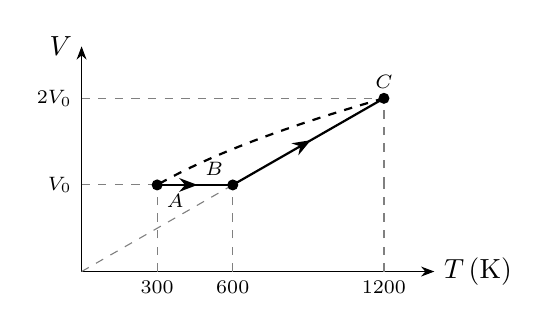
\begin{tikzpicture}[x=0.32cm,y=1.1cm,>=Stealth]
        \draw[->] (0,0) -- (14,0) node[right] {$T$\,(K)};
        \draw[->] (0,0) -- (0,2.6) node[left] {$V$};
        \draw[gray,dashed] (0,0) -- (6,1);
        \draw[gray,dashed] (0,1) node[left,black] {\scriptsize $V_0$} -- (3,1);
        \draw[gray,dashed] (0,2) node[left,black] {\scriptsize $2V_0$} -- (12,2);
        \foreach \t/\l in {3/300,6/600,12/1200}
          \draw[gray,dashed] (\t,0) node[below,black] {\scriptsize \l} -- (\t,1);
        \draw[gray,dashed] (12,1) -- (12,2);
        \draw[thick,->] (3,1) -- (4.6,1);
        \draw[thick] (4.5,1) -- (6,1);
        \draw[thick,->] (6,1) -- (9.1,1.517);
        \draw[thick] (9,1.5) -- (12,2);
        \draw[thick,dashed,domain=12:3,samples=40] plot (\x,{sqrt(\x/3)});
        \fill (3,1) circle (2pt) node[below right] {\scriptsize $A$};
        \fill (6,1) circle (2pt) node[above left] {\scriptsize $B$};
        \fill (12,2) circle (2pt) node[above] {\scriptsize $C$};
      \end{tikzpicture}\\
      {\small szaggatott: $C\to A$ (szorgalmi)}
      \end{minipage}
    \item Az óramutatóval ellentétes körüljárásnál \textbf{hűtőgép / hőszivattyú} lesz
      belőle. Ciklusonként $W = +150~\text{J}$ munkát kell befektetni (minden szakaszon
      megfordul $Q$, $W$, $\Delta E$ előjele).
  \end{enumerate}

\item
  \begin{enumerate}
    \item Hűlés $20\,^\circ$C-ról $0\,^\circ$C-ra:
      $Q_1 = c\,m\,\Delta T = 4180\cdot 0{,}5\cdot 20 = 41\,800~\text{J}$.\\
      Fagyás: $Q_2 = L_\text{o}\,m = 334\,000\cdot 0{,}5 = 167\,000~\text{J}$.\\
      Összesen: $Q = 208\,800~\text{J} \approx 209~\text{kJ}$.
    \item
      \begin{minipage}[t]{0.58\linewidth}
      Először rövid, ferdén csökkenő szakasz $20\,^\circ$C-ról $0\,^\circ$C-ra, majd hosszú
      vízszintes szakasz $0\,^\circ$C-on (fagyás). Állandó hőelvonásnál az idők a hőkkel
      arányosak: $167/41{,}8 \approx 4$, tehát a vízszintes szakasz kb.\ négyszer olyan
      hosszú.\\
      A vízszintes szakaszon a belső energia \textbf{csökken} (a molekulák kristályrácsba
      rendeződnek, a kötési energia felszabadul és ezt vonja el a fagyasztó), miközben a
      hőmérséklet állandó.
      \end{minipage}\hfill
      \begin{minipage}[t]{0.38\linewidth}\vspace{0pt}\centering
      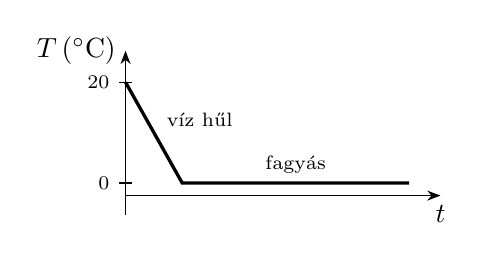
\begin{tikzpicture}[scale=0.8,>=Stealth]
        \draw[->] (0,0) -- (5,0) node[below] {$t$};
        \draw[->] (0,-0.3) -- (0,2.3) node[left] {$T$\,($^\circ$C)};
        \draw (0.1,0.2) -- (-0.1,0.2) node[left] {\scriptsize 0};
        \draw (0.1,1.8) -- (-0.1,1.8) node[left] {\scriptsize 20};
        \draw[very thick] (0,1.8) -- (0.9,0.2) -- (4.5,0.2);
        \node[above] at (2.7,0.2) {\scriptsize fagyás};
        \node[right] at (0.5,1.2) {\scriptsize víz hűl};
      \end{tikzpicture}
      \end{minipage}
    \item $W = \dfrac{Q_\text{fel}}{\varepsilon} = \dfrac{208\,800~\text{J}}{3} =
      69\,600~\text{J} \approx 70~\text{kJ}$.\quad
      $Q_\text{le} = Q_\text{fel} + W = 278\,400~\text{J} \approx 278~\text{kJ}$.
    \item Hideg tartály: a fagyasztó belseje, $T_\text{h} = 255~\text{K}$; meleg tartály:
      a hőleadó rács, $T_\text{m} = 313~\text{K}$.
      $\varepsilon_\text{max} = \dfrac{T_\text{h}}{T_\text{m} - T_\text{h}} =
      \dfrac{255}{58} \approx 4{,}4$. Mivel $3 < 4{,}4$, a fagyasztó nem sérti a
      II.~főtételt.
    \item Gyors folyamat, ezért \textbf{adiabatikus} közelítés: $Q = 0$ (nincs idő
      hőcserére); $W > 0$ (összenyomás); $\Delta E = W > 0$; $\Delta T > 0$.
    \item \textbf{Melegszik.} Nyitott ajtónál a gép a konyhából vonja el a $Q_\text{fel}$
      hőt, és a hátoldalán ugyanoda adja le a $Q_\text{fel} + W$ hőt. A konyha
      energiamérlege így $+W$: a felhasznált elektromos energia végül mind hővé alakul a
      konyhában.
    \item A hőerőgép a $40\,^\circ$C-os rács és a $20\,^\circ$C-os konyha között működne:
      $\eta_\text{max} = 1 - \dfrac{293}{313} = \dfrac{20}{313} \approx 6{,}4\%$.
      A $278{,}4~\text{kJ}$ leadott hőből így legfeljebb
      $0{,}064\cdot 278{,}4~\text{kJ} \approx 17{,}8~\text{kJ}$ munka nyerhető, a
      kompresszornak viszont $69{,}6~\text{kJ}$ kell, ennek alig negyede.\\
      Általánosan: ha működne, az egész berendezés külső munka nélkül szállítana hőt a
      hideg fagyasztóból a meleg konyhába. Ez a II.~főtételt sérti (Clausius-féle
      megfogalmazás), az energiamegmaradást nem: \textbf{másodfajú perpetuum mobile}
      lenne.
  \end{enumerate}
\end{enumerate}

\end{document}
